% !TeX root = ../main.tex
\section{Evaluation}
\label{sec:evaluation}
We evaluate whether faster vertex-pair updates reduce the time needed to obtain a layout of comparable stress~\cite{ref46}. The evaluation covers runtime and final stress relative to sequential CPU and lock-based GPU implementations after 15 iterations, elapsed SGD time to a shared stress target, a comparison of split and unsplit schedules on preferential-attachment graphs, and preprocessing-inclusive runtime for road networks with millions of vertices.

We ran each implementation separately on an Apple M4 Pro with 24 GiB unified memory and macOS 15.7.2.
CPU is sequential Rust with f64 arithmetic; Atomic uses native Metal, and both RoundRobin methods use Rust, wgpu, and WGSL~\cite{ref31} with the Metal backend and f32 updates.
The implementations differ in numerical precision and execution paths, so the measured speedups reflect these differences as well as scheduling.
Within each family, inputs, seeds, initial layouts, learning rates, and Sparse preprocessing are matched.
We remeasured RoundRobin Full SGD and retained the archived CPU, Atomic, and Sparse measurements from the same machine. These main comparisons combine different measurement dates and do not isolate transient system load. The additional preferential-attachment experiment measures CPU and both Full GPU schedules during the same session.
We use 15 iterations with Zheng et al.'s schedule~\cite{ref28}, $\epsilon=0.1$, five seeds for runtime comparisons, and ten for convergence diagnostics.
We fix Full at $T=1024$ with 16 segments and retain four alternating segments per phase in Sparse. Tile-size sensitivity is outside this evaluation.
We fix Sparse at 200 pivots in the CPU and GPU comparisons so that every method optimizes the same approximation. RoundRobin Full SGD and RoundRobin Sparse SGD workgroups contain 1024 and 256 threads, respectively.

We evaluated Full SGD on 20 graphs and Sparse SGD on 38, using datasets based on the SuiteSparse collection~\cite{ref6}.
For \graph{com-Amazon}, \graph{com-DBLP}, and \graph{loc-Gowalla}, all compared methods use the same official SNAP inputs.
We remove directions, weights, numerical zeros, self-loops, and duplicate edges, and verify identical preprocessed largest connected components by SHA hashes.
The comparisons use a 120-second process threshold and an observed 8-GiB RSS threshold, sampled approximately every 200 ms.
A stopped preliminary run prevents formal runs for that setting; failed, unlaunched, and unavailable runs are excluded from paired ratios, rather than assigned artificial values.
RSS monitoring is not a strict instantaneous or dedicated-GPU-memory limit.

SGD time includes shuffling, dispatch, completion waits, and resubmission, but excludes preprocessing, initialization, stress evaluation, and coordinate saving.
For runtime comparisons we divide the 15-iteration total by 15; the road-network experiment reports the total.
Algorithm time additionally includes preprocessing, GPU setup, transfers, and postprocessing; process time also includes input, evaluation, and output.
Quality comparisons use the full stress objective in \eqref{eq:stress}, computed exactly up to 8,000 vertices and otherwise estimated from 256 fixed sources independent of the pivots.
For jointly successful seeds, speedup is CPU time divided by GPU time, and stress ratio is GPU stress divided by CPU stress.
We report graph-level medians, with seed minima and maxima rather than confidence intervals.

\subsection{Comparison with CPU and Atomic}
\label{sec:comparison}
\begin{figure*}[!t]
\centering
\includegraphics[width=\textwidth]{fig05_comparison.pdf}
\caption{Mean time per iteration for sequential CPU, Atomic GPU, and RoundRobin GPU SGD. For each seed we divide the SGD time by 15. Symbols show the median and bars the range over seeds completed by all three methods (95 Full and 179 Sparse triples). N/A marks graphs without a complete triple. The vertical axis is logarithmic.}
\label{fig:comparison}
\end{figure*}

Using $T=1024$ for Full and $p=200$ for Sparse, \autoref{fig:comparison} compares mean iteration times for each graph. We also report final stress ratios to assess layout quality.

RoundRobin Full SGD is faster on 17 of 19 comparable graphs, with median speedups of $0.855$--$23.469\times$.
The two slowdowns occur on \graph{dwt_1005} and \graph{1138_bus}.
For \graph{fe_4elt2}, speedup is $23.469\times$ with a stress ratio of 1.010; for \graph{wiki-Vote}, the values are $16.928\times$ and 1.026.
Eighteen graphs have a median stress ratio at most 1.05, and sixteen combine this quality criterion with faster iterations. The remaining quality gap is on \graph{bcsstk17}, whose ratio is 1.208.
Atomic is faster on 13 of 19 graphs, with speedups of $0.064$--$3.365\times$ and stress ratios of 1.001--2.921.
Its recording of pair-update order and pre-update coordinates contributes work beyond locking, so the difference between RoundRobin and Atomic is not a measurement of lock overhead alone.

\begin{figure*}[!t]
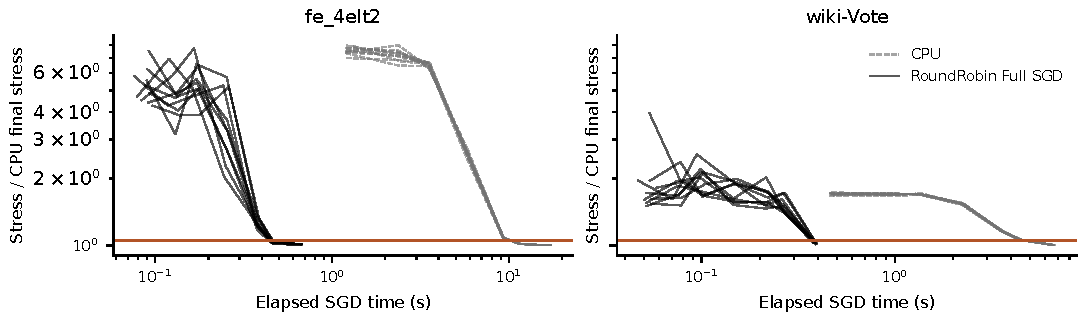
\includegraphics[width=\textwidth]{full_time_to_quality.pdf}
\caption{Full SGD diagnostic runs, ten seeds per method. Each trace joins saved checkpoints from iteration 1 to 15 for one seed. Stress is relative to that seed's final CPU stress. The horizontal line marks the 1.05 target.}
\label{fig:full-time}
\end{figure*}
On both \graph{fe_4elt2} and \graph{wiki-Vote}, all ten RoundRobin traces reach the target (\autoref{fig:full-time}). Their median attainment times are 0.463 and 0.385 s, compared with CPU times of 11.593 and 6.691 s.

RoundRobin Sparse SGD is faster on all 37 comparable graphs, with speedups of $6.136$--$55.053\times$ and stress ratios of 0.987--1.067.
Thirty-six graphs combine faster execution with a stress ratio at most 1.05.
Atomic is faster on two of 37 graphs: its speedups are $0.869$--$1.042\times$ and stress ratios 0.971--1.139.
Only one graph combines Atomic acceleration with a stress ratio at most 1.05.

Of 100 planned Full runs per method, CPU completed 95 (five memory stops), Atomic completed 95 (five withheld after preliminary failure), and RoundRobin Full SGD completed all 100.
Of 190 Sparse runs per method, CPU completed 181 and Atomic 180. Both withheld five after preliminary failure and had three memory stops. CPU had one additional timeout and Atomic two. RoundRobin Sparse SGD completed all 190. The pairwise ratios above use every seed completed by CPU and the GPU method under comparison. For the three-way plot in \autoref{fig:comparison}, we require all three methods to complete the same seed.

\begin{figure*}[t]
\centering
\includegraphics[width=\textwidth]{full_degree_scaling.pdf}
\caption{Full SGD on preferential-attachment graphs. Each vertex count has two graph seeds; points are medians and bars are minima and maxima over five matched initial layouts. (a) Mean iteration time on a logarithmic axis. (b) Exact final stress relative to same-seed CPU stress. The horizontal line marks 1.05. Both GPU variants use the same update rule, tile size, and per-iteration completion wait.}
\label{fig:degree}
\end{figure*}

\subsection{Convergence toward a Quality Target}
\label{sec:convergence}

The Sparse convergence runs retain the 200 pivots from the timing comparison. Changing the pivot set here would change the objective as well as the trajectory toward the target. We save layouts at iterations 0, 1, 2, 3, 5, 8, 10, and 15 while retaining the same learning-rate schedule.
The target is at most 1.05 times the same-seed CPU final stress.
We apply the same threshold to the CPU checkpoints. \autoref{tab:arrival} reports the first saved checkpoint at or below the target for each seed. Times exclude saving and intermediate readback.

\begin{table}[tb]\centering
\caption{Observed attainment within 15 iterations. Each row has ten paired seeds. Hit and End count RoundRobin runs reaching the target at any checkpoint and at iteration 15, respectively. Times are median cumulative SGD seconds at first observed attainment. CPU reached the target on all seeds. The RoundRobin time uses successful seeds only.}
\label{tab:arrival}
\small
\begin{tabular}{@{}lrrrr@{}}\toprule
Graph & Hit & End & CPU (s) & RR (s)\\ \midrule
\multicolumn{5}{l}{Full}\\
\graph{USpowerGrid} &10&10&2.046&0.199\\
\graph{dwt_2680} &6&6&0.807&0.160\\
\graph{bcsstk16} &10&10&2.907&0.285\\
\graph{fe_4elt2} &10&10&11.593&0.463\\
EVA &9&9&1.678&0.281\\
\graph{wiki-Vote} &10&10&6.691&0.385\\
\midrule
\multicolumn{5}{l}{Sparse}\\
\graph{luxembourg_osm} &10&10&6.722&0.149\\
\graph{kron_g500-logn18} &10&10&2.138&0.919\\
\graph{coAuthorsCiteseer} &10&10&13.925&0.391\\
\bottomrule\end{tabular}
\end{table}

Across the six Full graphs, 55 of 60 runs attain the target and 55 remain within it at iteration 15. The five Full misses occur on \graph{dwt_2680} (four seeds) and EVA (one seed), so segmentation does not guarantee the target for every initialization. All 30 Sparse runs attain it and remain within it at iteration 15.
The recorded checkpoints bound the first observed attainment; they do not identify the exact crossing between saved iterations.

\begin{figure*}[!t]
\centering
\includegraphics[width=0.90\textwidth]{fig07_large_layouts.pdf}
\caption{RoundRobin Sparse SGD layouts of Italy and Germany with 40 pivots, 15 iterations, and seed 0. All vertices and edges are rendered; panels preserve aspect ratio but use independent scales. Color encodes normalized BFS distance from the lowest-ID vertex. Geographic coordinates are not used.}
\label{fig:large}
\end{figure*}

\paragraph{Degree heterogeneity and graph size.}
We generated six Barab\'asi--Albert preferential-attachment graphs using NetworkX: 2,000, 4,000, and 8,000 vertices, five attachments per new vertex, and graph seeds 0 and 1 at each size.
The edge counts are 9,975, 19,975, and 39,975, respectively; maximum degrees range from 143 to 311.
For each graph, we use five matched initial layouts (seeds 0--4), exact full stress, and the same 15-iteration schedule.
We measure CPU, unsplit RoundRobin Full SGD, and the 16-segment schedule sequentially, alternating method order across initialization seeds after a preliminary run for each setting.
Both GPU schedules wait for completion at each iteration, isolating segmentation from the earlier change in CPU wait placement.
Across these six graphs, median CPU speedups range from $2.96$ to $22.95\times$ for 16 segments.
Unsplit final stress ratios range from 1.170 to 1.519, compared with 1.007 to 1.038 after segmentation (\autoref{fig:degree}).
Of the 30 matched layouts, 0 unsplit runs and 30 split runs finish within 5\% of CPU.
The split schedule takes 1.16--1.42 times the unsplit iteration time in graph-level medians.
These measurements show the time--quality effect of interleaving within this graph family; they do not isolate degree distribution from other structural properties or establish behavior on all networks.

\subsection{Scaling to Road Networks with Millions of Vertices}
\label{sec:large}

Beyond the CPU comparisons, we run RoundRobin Sparse SGD on \graph{italy_osm} and \graph{germany_osm}, with 6,686,493 and 11,548,845 vertices and 7,013,978 and 12,369,181 undirected edges, respectively.
Both runs use 40 pivots, 15 iterations, $\epsilon=0.1$, and seed 0 on the same GPU, without the comparison experiments' stopping thresholds.
We use the same reduced count for both networks to compare their runtimes under one memory budget. For Germany, storing one 32-bit distance for each vertex and pivot requires 1.72 GiB at 40 pivots, 8.60 GiB at 200, and 44.06 GiB at 1024. The last figure exceeds the laptop's 24 GiB of unified memory even before coordinates and other buffers.
There are no paired CPU or Atomic runs at these scales.

\begin{table}[!t]
\centering
\caption{Road-network runtime in seconds (one run per graph). SGD is the total for 15 iterations; algorithm time also includes preprocessing, setup, transfers, and postprocessing, but excludes input loading, stress evaluation, saving, and rendering.}
\label{tab:large}
\begin{tabular}{@{}lrr@{}}
\toprule
Graph & SGD (s) & Algorithm (s)\\
\midrule
\graph{italy_osm} & 2.11 & 43.45\\
\graph{germany_osm} & 4.48 & 80.32\\
\bottomrule
\end{tabular}
\end{table}
Both layouts complete (\autoref{fig:large}; \autoref{tab:large}).
Germany takes 4.48 s for 15 iterations and 80.32 s including preprocessing and other algorithm work, demonstrating a completed layout beyond ten million vertices on one GPU.
The largest verified input is not a measured capacity limit, and these 40-pivot runs do not establish equivalence to 200-pivot quality or CPU speedups.
Preprocessing and data handling dominate overall time and remain important optimization targets.

The distinction between SGD time and algorithm time is especially important at this scale.
SGD accounts for approximately 4.9\% of algorithm time for Italy and 5.6\% for Germany.
Thus, accelerating the pair-update kernels further would address only a small part of the current time to produce coordinates.
Common preprocessing alone took 37.50 s for Italy and 68.51 s for Germany. Both runs also evaluated full stress separately using 64 sampled sources, yielding $8.93\times10^{11}$ and $1.46\times10^{12}$, respectively. These absolute values describe different graphs and do not quantify the quality cost of reducing the pivot count. The run records contain no peak-memory measurement for either layout.

The pivot count provides a separate control over the size of the sparse problem.
With fixed $p$, the $O(m+np)$ term count grows linearly with the numbers of edges and vertices.
More pivots would represent long-range distances from more reference vertices. A larger-pivot experiment on a graph that fits in memory could test whether this improves full stress enough to justify its cost. Reducing $p$ from 200 to 40 reduces the vertex--pivot term budget by a factor of five, while leaving the actual-edge terms in place.
It changes the sparse objective as well as storage and work, so the large-road experiment demonstrates feasibility under a stated configuration rather than extrapolating the CPU comparison results.
The two completed runs establish a concrete operating point beyond ten million vertices; determining a maximum graph size would require a systematic sweep over graph structure, pivot count, and memory use.
